\chapter{Software}
\label{chapter:software}

In this chapter, we describe the technical details of the software tools we developed for the control of Boolean networks. We first give an overview of the software. Then we describe the implementation underlying backend details of the main components of the software. Finally, we describe the python package and the web application that we developed to make the software accessible to a wider audience.

\section{Software overview}
\label{sec:software_architecture}

The software for the control of \PBN{} networks was developed as part of the BioDivine tools\footnote{\url{https://sybila.fi.muni.cz/tools.html}} developed by the Sybila~\footnote{\url{https://sybila.fi.muni.cz/index.html}} (Systems Biology Laboratory) research group at Masaryk University. 

The tools were initially oriented on a ``colored model checking'' of parametrized continuous models of biological systems~\cite{Brim2015}. The approach was also later extended to hybrid models~\cite{Smijakova2020}. The main idea behind colored model checking was encoding the continuous models as discrete color-labelled transition systems, and then applying SMT model checking techniques to analyze their behavior. This approach also enabled solving the parameter synthesis and attractor bifurcation problems for these models~\cite{Benes2016,Benes2017}.

Building on top of the previous work, the group shifted focus from discretized continuous models to Boolean networks, which are a more direct ``natively'' discrete modeling formalism. The former parameters of continuous models and their paramters synthesis was reoriented from continuous values of parameters to unknown functions of the network structure.

At first, the tools were mostly focused on the bifurcation analysis of \PBN{}~\cite{Benes2019}. To nurture the adoption of the tool, a web application was developed to make the tool accessible to a wider audience~\cite{aeon}. The web application allowed users to upload their own partially specified Boolean network models, adjust them and run the bifurcation analysis. 

Since globally there was not a lot of tools supporting analysis of \PBN{} models, the Aeon tools were extended to support also other types of analysis. In particular, we implemented the control of \PBN{} models, which is the main topic of this thesis. The control of \PBN{} models was implemented as a new component of the software, and it was integrated into the web application as well. 

Later, to make the control of \PBN{} models more accessible to users who prefer working with code, we also implemented a python package that provides an interface to the control algorithms implemented in the software~\cite{aeonpy}. The tool also provides all underlying algorithms and data structures such as the symbolic representation of the state space, and the algorithms for computing the attractors and their basins of attraction. The tool is also being extended by higher-level algorithms for the analysis of \PBN{} models, such model checking of temporal properties, and the analysis of the structure of the state space~\cite{Benes2023,Benes2024bnclassifier}.

\begin{figure}[htbp]
    \centering
    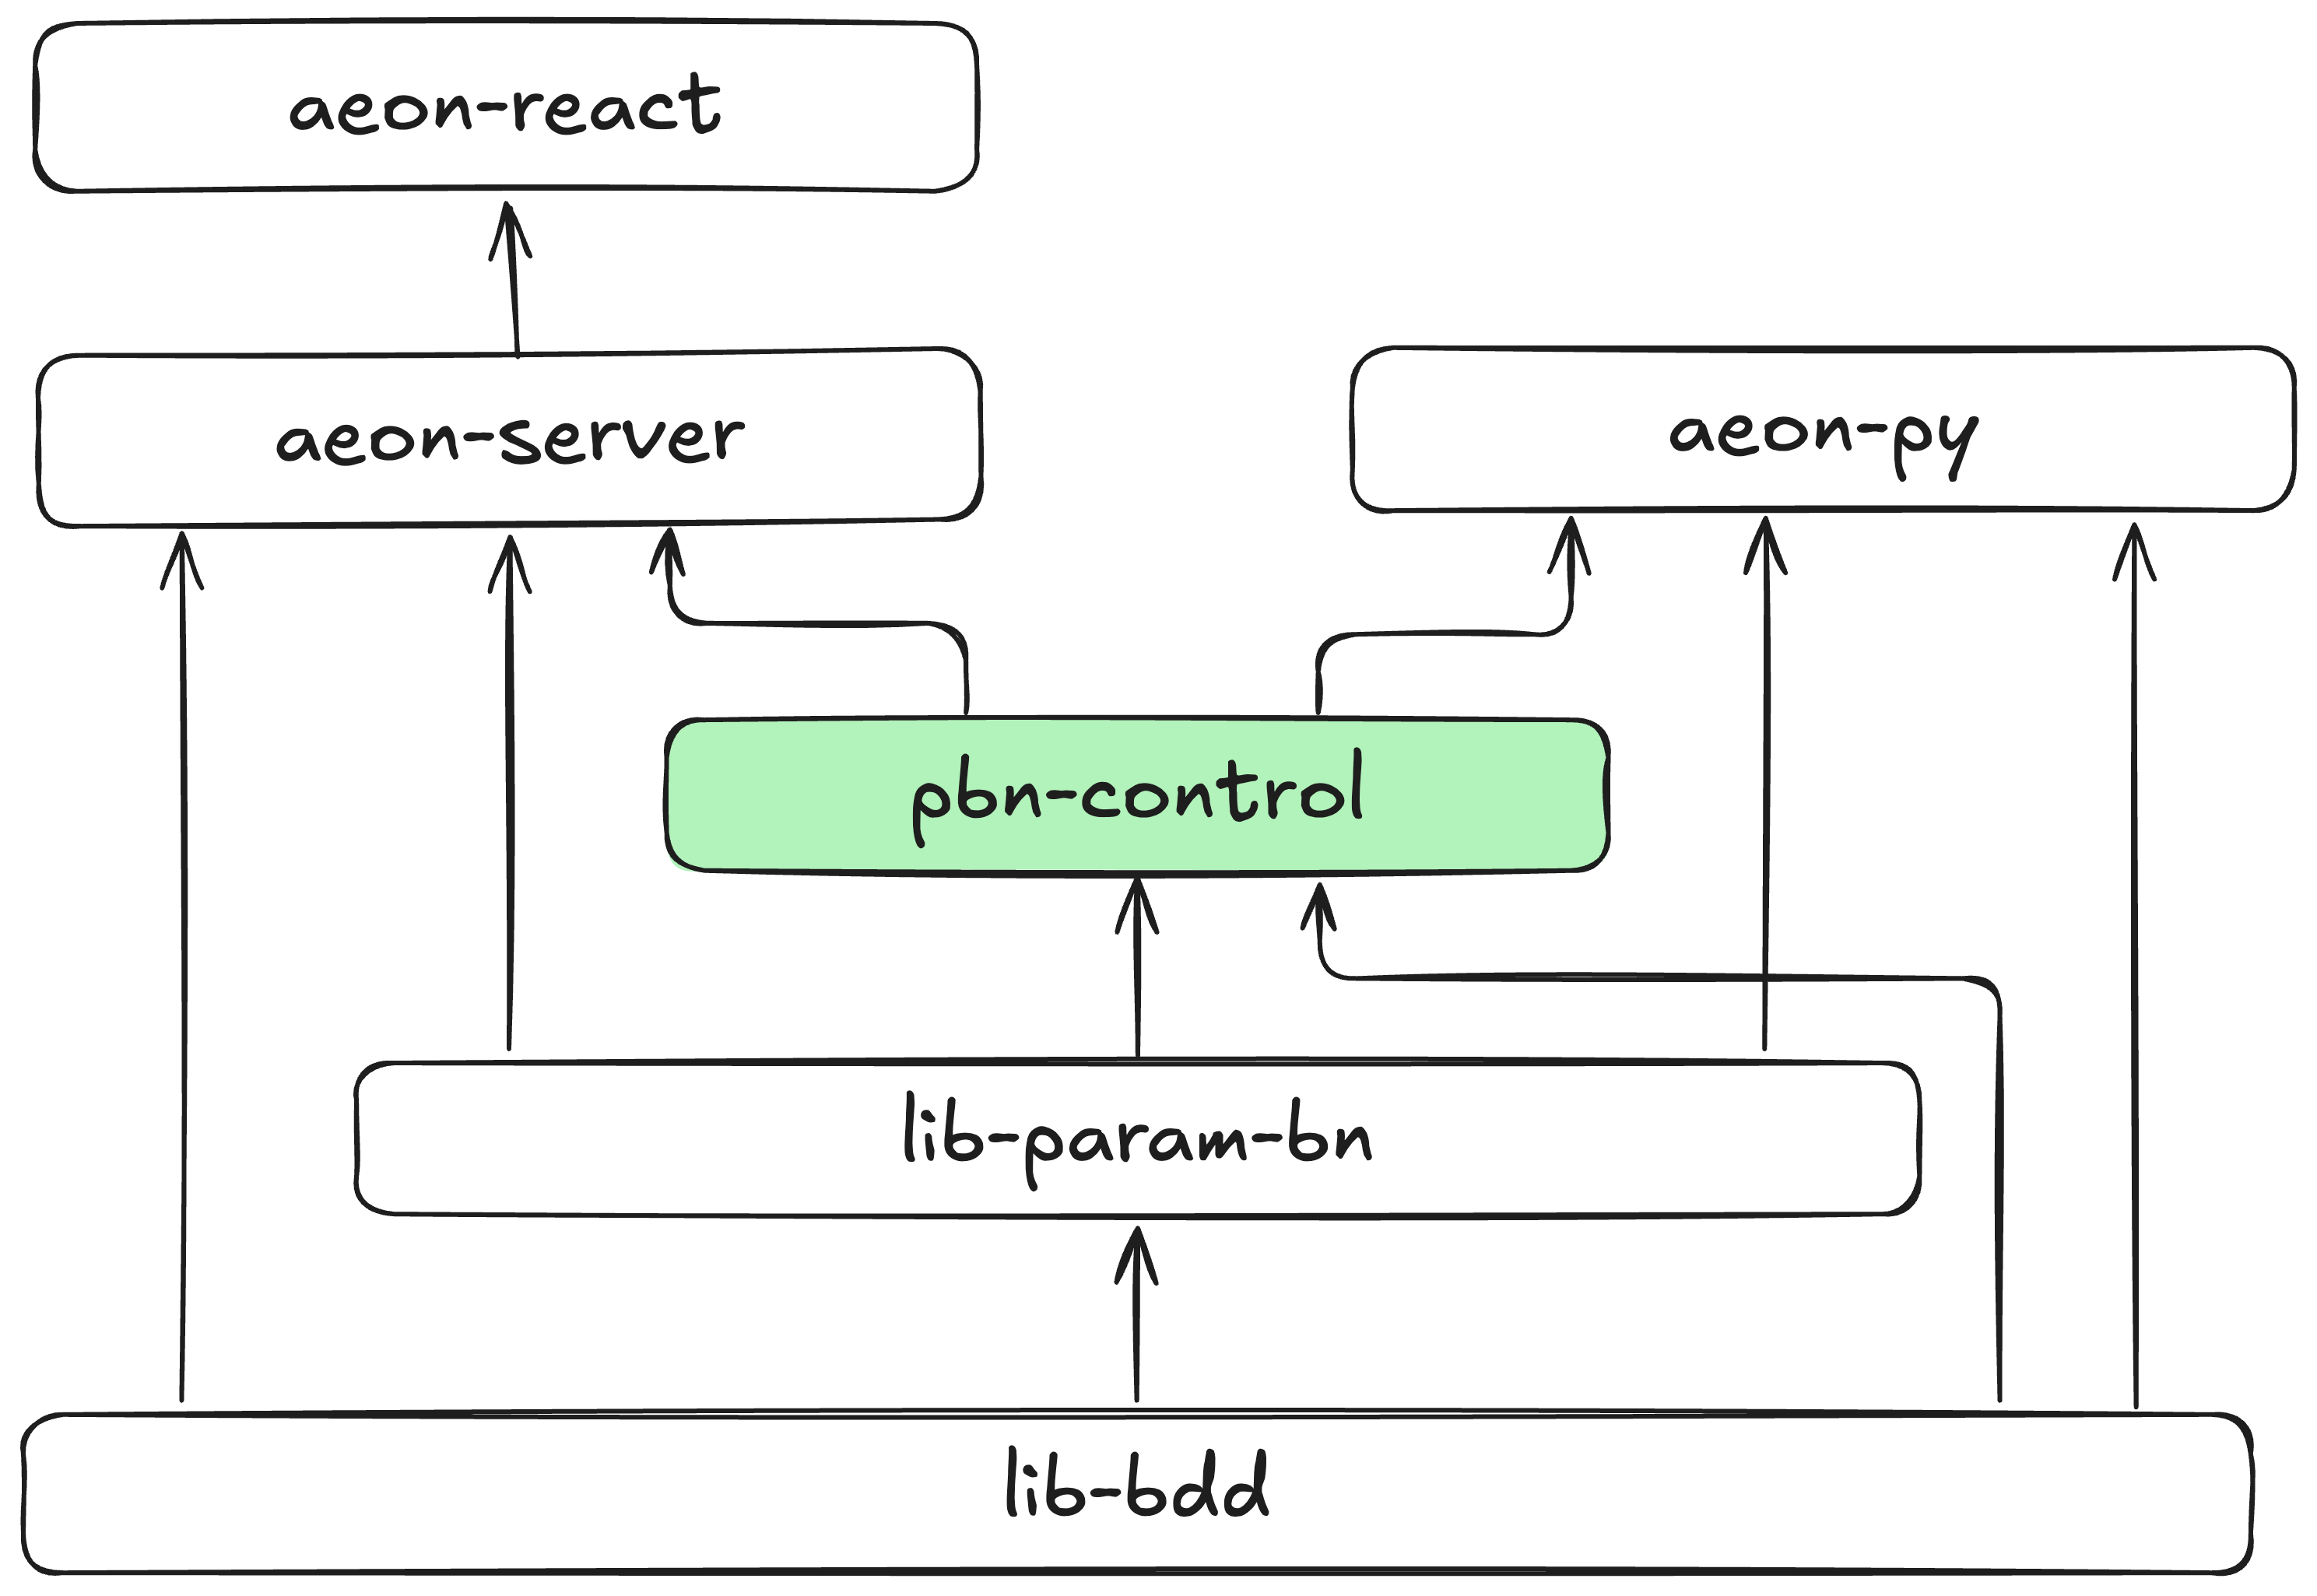
\includegraphics[width=0.8\textwidth]{Figures/sw_arch.png}
    \caption{
        \textbf{Biodivine Aeon software architecture overview.} The figure depicts components of the biodivine software related to the control of Boolean networks. The green box represents the main Rust library, which contains the core algorithms and data structures for Boolean network control. The arrows indicate the dependencies between the components. 
    }
    \label{fig:sw_arch}
\end{figure}

In \autoref{fig:sw_arch}, we give an overview of the software architecture of the Aeon tools. The core components are implemented in Rust language because of its performance, memory safety and mature developer experience. Component lib-bdd is the low-level library for the symbolic representation of the state space using binary decision diagrams (BDDs). It is independent of Boolean networks and can be used for any application that requires symbolic representation of state spaces. 

Component lib-param-bn is the main library for the performant analysis of \PBN{} models, which contains the algorithms for computing attractors, reachability algorithms and bifurcation. On top of the two libraries, we implemented the control of \PBN{} models as a new component of the software. Since the control of \PBN{} requires custom encoding of the perturbations it also relies on the lib-bdd library for the symbolic representation of the state space. The control component also relies on the lib-pbn library for computing the attractors and their basins of attraction, which are used in the control algorithms.

Finally, we implemented a web application that is built on top of all the rust components. Aeon-server provides a server functionality such as validation of the uploaded models and progress reporting to interact with the software through a web interface. The web application (aeon-react) than uses just the server component of the software, which provides an API for the users to interact with the software through the web interface. Later, also a python package aeon-py was implemented to provide a convenient python interface for all low-level algorithms and data structures. 

\section{Core packages}
\label{sec:core_packages}

\paragraph{lib-bdd} The lib-bdd library provides a symbolic representation of the state space using binary decision diagrams (BDDs). It provides basic operations for manipulating BDDs, such as conjunction, disjunction, negation, and quantification. 

Compared to many other implementations, each Binary Decision Diagram (BDD) instance manages its own memory. This design simplifies serialization and enables safe sharing between threads, which is particularly beneficial for applications that process large numbers of BDDs concurrently. It also aligns well with the ownership and safety principles emphasized in the Rust programming language.

The implementation provides support for a range of common operations on BDDs. These include standard logical operations, evaluation of Boolean expressions, and transformations between BDD representations and conjunctive or disjunctive normal forms. Additional functionality allows inspection of BDD structures, conversion back to Boolean expressions, and visualization through graph exports. The system also supports several relational-style operations commonly used in symbolic computation, such as projection and restriction. Note that these operations were used in \autoref{subsec:symbolic_ops} and \autoref{sec:phen_control_method} for the control of \PBN{} models.

\paragraph{lib-param-bn} The lib-param-bn library is the main library for the performant analysis of \PBN{} models, which contains the algorithms for computing attractors, reachability algorithms and bifurcation. In particular, it implements fully \emph{symbolic} representation of the state space of \PBN{} models using BDDs, that can combine interpretations and states in a single BDD. 

This library was used to provide all reachability, trap set and attractor computations for the control algorithms implemented in this thesis that are described in \autoref{subsec:supporting_algos} and \autoref{sec:phen_ctrl_algo}.

Previously the library used semi-symbolic representation of the state space, where only interpretations were represented symbolically, while states were represented explicitly. This approach was used in the initial version of the control algorithms implemented in this thesis, which are described in \autoref{ss:semi_symbolic_sb}.

\paragraph{pbn-control} The pbn-control library provides the necessary functionality for the control of \PBN{} models, including the implementation of various control strategies and algorithms.

In particular, it implements the encoding of perturbations as function symbols (parameters), that are added to the original \PBN{} model. This allows us to use the same symbolic representation of the state space for both the original model and the perturbations, which is crucial for the performance of the control algorithms. The library also implements the algorithms for computing the control and manipulating with the control map relations, which are used in the control algorithms described in \autoref{ss:control_algos_st_otp} and \autoref{sec:phen_ctrl_algo}.

Since we have shown, that symbolic one-step control is superior to semi-symbolic one-step control, the current version of the control algorithms implemented in the software relies on the fully symbolic representation of the state space provided by the lib-param-bn library. However, the initial version of the control algorithms implemented in this thesis, which are described in \autoref{ss:semi_symbolic_sb}, relied on the former semi-symbolic representation of the state space.

\section{Aeon web application}
\label{sec:aeon_web_app}

Aeon web application is a web-based interface for the analysis of \PBN{} models. It allows users to upload their own models, adjust them and run various analyses, including the control of \PBN{} models. The initial version of the web application was developed to make the bifurcation analysis of \PBN{} models accessible to a wider audience. The initial version was first released in 2020~\cite{aeon}. 

In version 0.5.0 of the web application, we integrated the control of \PBN{} models as a new component of the software~\cite{Vesely2025}. During implementation of the new control module, it was discovered, that technical debt in the codebase of the web application was making it difficult to implement the new control module. Therefore, it was decided to refactor the web application to make it more modular and maintainable. This has led to a major refactor of the web application, which was released in version 0.6.0 and which is also briefly presented here.

\begin{figure}[htbp]
    \label{fig:sw_load_model}
    \centering
    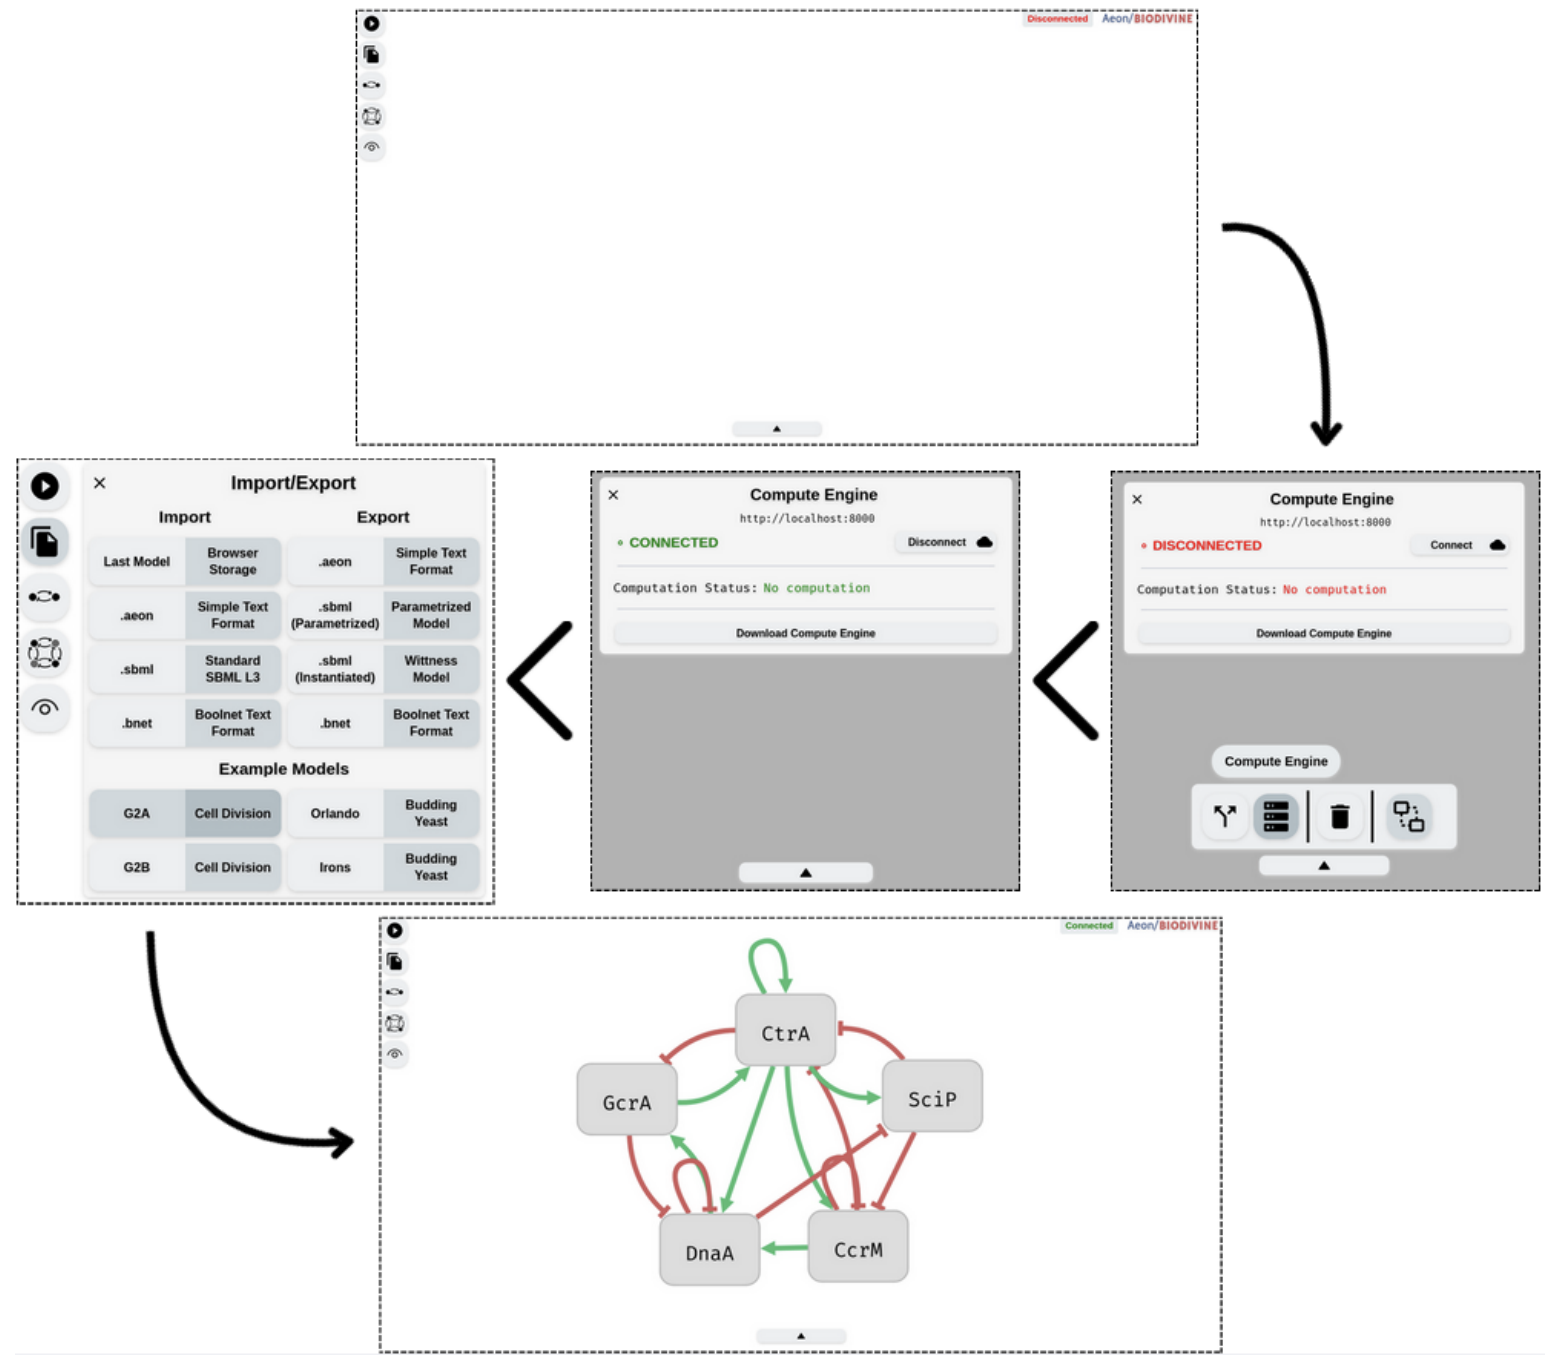
\includegraphics[width=\textwidth]{Figures/aeon_load_model.png}
    \caption{
        \textbf{Biodivine Aeon web application interface.} From~\cite{Vesely2026}. The figure shows the main interface of the Aeon web application, where users can upload and load their own \PBN{}.
    }
\end{figure}

AEON tool is available at \url{https://biodivine.fi.muni.cz/aeon/} as an online tool. Due to the potential high computational complexity of the analyses, SyBiLa group does not provide a public instance of the web application server, but instead provides a downloadable version of the server that users can run on their own machines.

The main flow of how a model can be uploaded and analyzed in the web application is shown in \autoref{fig:sw_load_model}. The user first needs to download and run the server component of the software on their own machine. Then, they can access the web application functionality through a web browser. The user can upload their own \PBN{} model in the form of a text file, which is then validated by the server or select one of the example models provided by the web application. Once the model is loaded, the user can adjust the model by changing the model functions, or by changing the regulations of the model.


\begin{figure}[htbp]
    \centering
    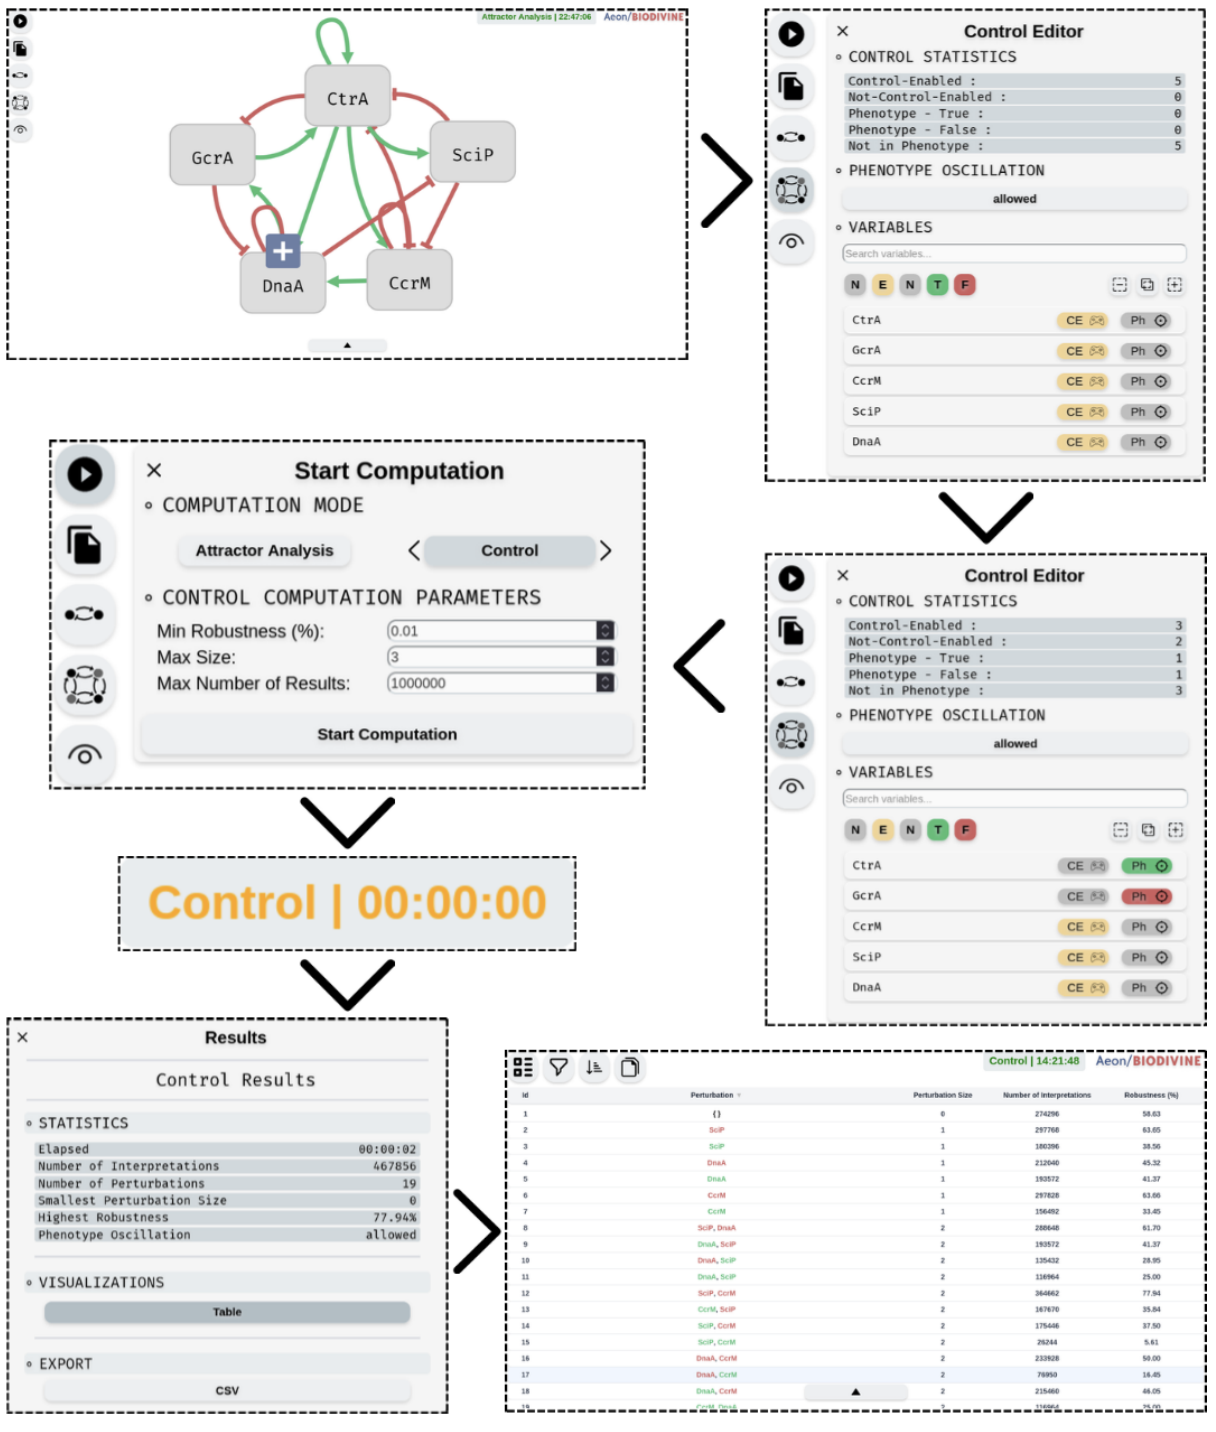
\includegraphics[width=\textwidth]{Figures/aeon_control.png}
    \caption{
        \textbf{Biodivine Aeon web application control interface.} From~\cite{Vesely2026}. The figure shows the control interface of the Aeon web application, where users can control their own \PBN{}.
    }
    \label{fig:sw_control}
\end{figure}


After the model is loaded, the user can run various analyses on the model, including the permanent phenotype control of \PBN{} models. The source-target control is not support via Aeon UI. It could be implemented later if there is a user interest. The control interface of the web application is shown in \autoref{fig:sw_control}. The user can select variables that can be perturbed, the type of the phenotype control (allowed, required or forbidden oscillation) and the target phenotype that they want to reach. The user can also adjust the parameters of the control algorithm, such as the minimal required robustness, maximum number of perturbations allowed or maximum number of results. 

After the control algorithm is run, the results are displayed in the web application, where the user can inspect the results and download in a CSV format for further analysis. The results include the comprehensive statistics about the control problem, such as elapsed time, number of interpretations that can be controlled, the number of perturbations found, highest robustness achieved, and other relevant information. Moreover, a full list of all possible perturbations that can be applied to reach the target phenotype is also available. The list can be filtered and sorted by various criteria, such as the number of perturbations, the robustness of the perturbation, or the variables that are perturbed. 

\section{Aeon.py}
\label{sec:python_package}

Since it can be difficult to develop a web application that covers all the functionality of the a very technical software, we also implemented a python package that provides an interface to the control algorithms implemented in the software~\cite{aeonpy}. The python package is available on PyPI and as part of the CoLoMoTo docker image~\cite{Naldi2015}. 

The CoLoMoTo toolset provides a robust and reproducible computational framework for the analysis of Boolean networks, enabling both qualitative and formal investigation of complex biological regulatory systems. Its Jupyter environment based on Docker ensures interoperability and reproducibility while facilitating scalable exploration of state-space dynamics under different updating schemes. Since it is widely used in the community of Boolean network modeling, we decided to make the Aeon control algorithms available as part of the CoLoMoTo docker image. This allows users who are already using the CoLoMoTo toolset to easily integrate the control algorithms into their existing workflows.

The python package provides a convenient interface for users who prefer working with code rather than a web application. It allows users to load their own \PBN{} models, adjust them and run the control algorithms directly from their python and run a large scale experiments programmatically.


\section{Summary}
In this chapter, we described the software tools we developed for the control of Boolean networks. We gave an overview of the software architecture and the main components of the software, including the core libraries for symbolic representation of state spaces and the control algorithms. We also described the web application that we developed to make the software accessible to a wider audience, and the python package that provides a convenient interface for users who prefer working with code. The software is available online and can be used by researchers interested in analyzing and controlling Boolean network models. In the next chapter, we will demonstrate the use of the software on a case studies with real-world applications.